%************************************************
\chapter{Introduction}
\label{chp:Introduction}
%************************************************

%\section{Motion Vision}
%what is motion vision. what is the central question we want to answer ? Why do we try to answer above question using drosophila ?

\section{\protect\NoCaseChange{\textit{Drosophila}} as a model organism}
\textit{Drosophila melanogaster} is one of the most powerful model organisms available for the functional dissection of neural circuits. It allows for sophisticated \textit{in vivo} neural manipulations that includes imaging, activation, and suppression of neural activity. The \textit{Drosophila} research community has developed thousands of 'driver-lines' that can be used to express genes of interest in a neuron-specific manner \parencite{Pfeiffer2008}. Additionally, \textit{Drosophila} offers several practical advantages: fruit flies are small, have a short generation time of about 10 days, and are easy to grow in the lab. 

The \textit{Drosophila} brain is estimated to contain only about 200,000 neurons \parencite{Raji2021} but produces behavior of rich complexity \parencite{Card2008, Pavlou2013, Ryu2022}. In systems neuroscience, a common goal is to understand how the brain processes and extracts relevant information from the sensory inputs to produce behavior. \textit{Drosophila} constitutes an ideal model organism to study the neural circuits and computations underlying behavior. Given some surprising parallels between how the fly and mammalian brains process information \parencite{Borst2015}, insights about the nervous system obtained in \textit{Drosophila} often might be relevant for understanding the brain of other species \parencite{Bellen2010}.
%It involves computation of modest complexity. These computations are implemented in circuits that contain a limited number of neurons, and with \textit{Drosophila} genetic armoury almost each of these neurons can be precisely targeted. However, even with comparatively little or less complexity, there are 
\section{Tools for functional dissection of \protect\NoCaseChange{\textit{Drosophila}} neural circuits}
To have a detailed understanding of how a neural circuit functions, the role each individual neuron plays in that particular circuit needs to be known. To achieve this, the following three types of manipulations can be performed on the given neuron: (i) record neuronal activity, (ii) activate the neuron, and (iii) silence the neuron. Fortunately, decades of research in \textit{Drosophila} have provided multiple tools that allow for these manipulations in the choice of the neuron. The most important tool that enables to do this in a neuron-specific manner is the Gal4-UAS system (figure \ref{fig:gal4uas}). 

\subsection{Targeting cell types: Gal4-UAS}
Following the discovery of transposable DNA sequences (P-elements) in the \textit{Drosophila} genome \parencite{Rubin1982}, the Gal4-UAS system was designed \parencite{Brand1993}. The Gal4-UAS system is a binary expression system consisting of two main components: the yeast transcriptional factor Gal4 expressed in a specific pattern, and a reporter gene under the control of a upstream activation sequence (UAS) promoter that is silent in the absence of Gal4. The Gal4-UAS system involves crossing two fly lines: one called the 'driver-line', defines which neurons express the required effector gene; the other called 'reporter-line', defines what gene is expressed in the neurons defined by the driver line (figure \ref{fig:gal4uas}). 

Another independent binary transcriptional system that can be used is the LexA-lexAop system. This method is based on the bacterial DNA-binding operator lexAop and controlled by the expression of LexA. The LexA binds to and activates the lexA operator (lexAop). The LexA-lexAop system can be used in combination with the Gal4-UAS system to simultaneously express two different genes in two different neuronal populations. %Using a combination of the GAL4-UAS and LexA-lexAop system, one can express the following three types of reporter genes: Indicator, Suppressor \& Activator.

Initially, the Gal4 fly lines were created by injecting randomly integrating P-elements transposons into the Drosophila embryos. However, the lack of control over specific insertion sites often resulted in broader expression patterns, making them unsuitable for circuit manipulations. Currently, DNA fragments with presumed enhancer activity are directly cloned for increased efficacy, and intersectional strategies, such as the split-Gal4 are used for increased specificity \parencite{Pfeiffer2008, Jenett2012}. In this method, the coding region of the Gal4 is split into two units: (i) the Gal4 activating domain (AD), and (ii) the Gal4 DNA binding domain (DBD). The expression of the Gal4-AD is under the control of one enhancer and the expression of the Gal4-DBD is under the control of another enhancer. The DBD and AD proteins alone are not able to promote gene expression; only cells where both enhancers are active produce functional Gal4 protein. Therefore, only in cells containing both subunits, the gene of interest is expressed \parencite{Luan2006}. Thousands of fly lines have been generated as a result, and nearly every type of fly neuron can be targeted with high specificity \parencite{Pfeiffer2010}.
\begin{figure}
\centering
\hspace*{-1cm} 
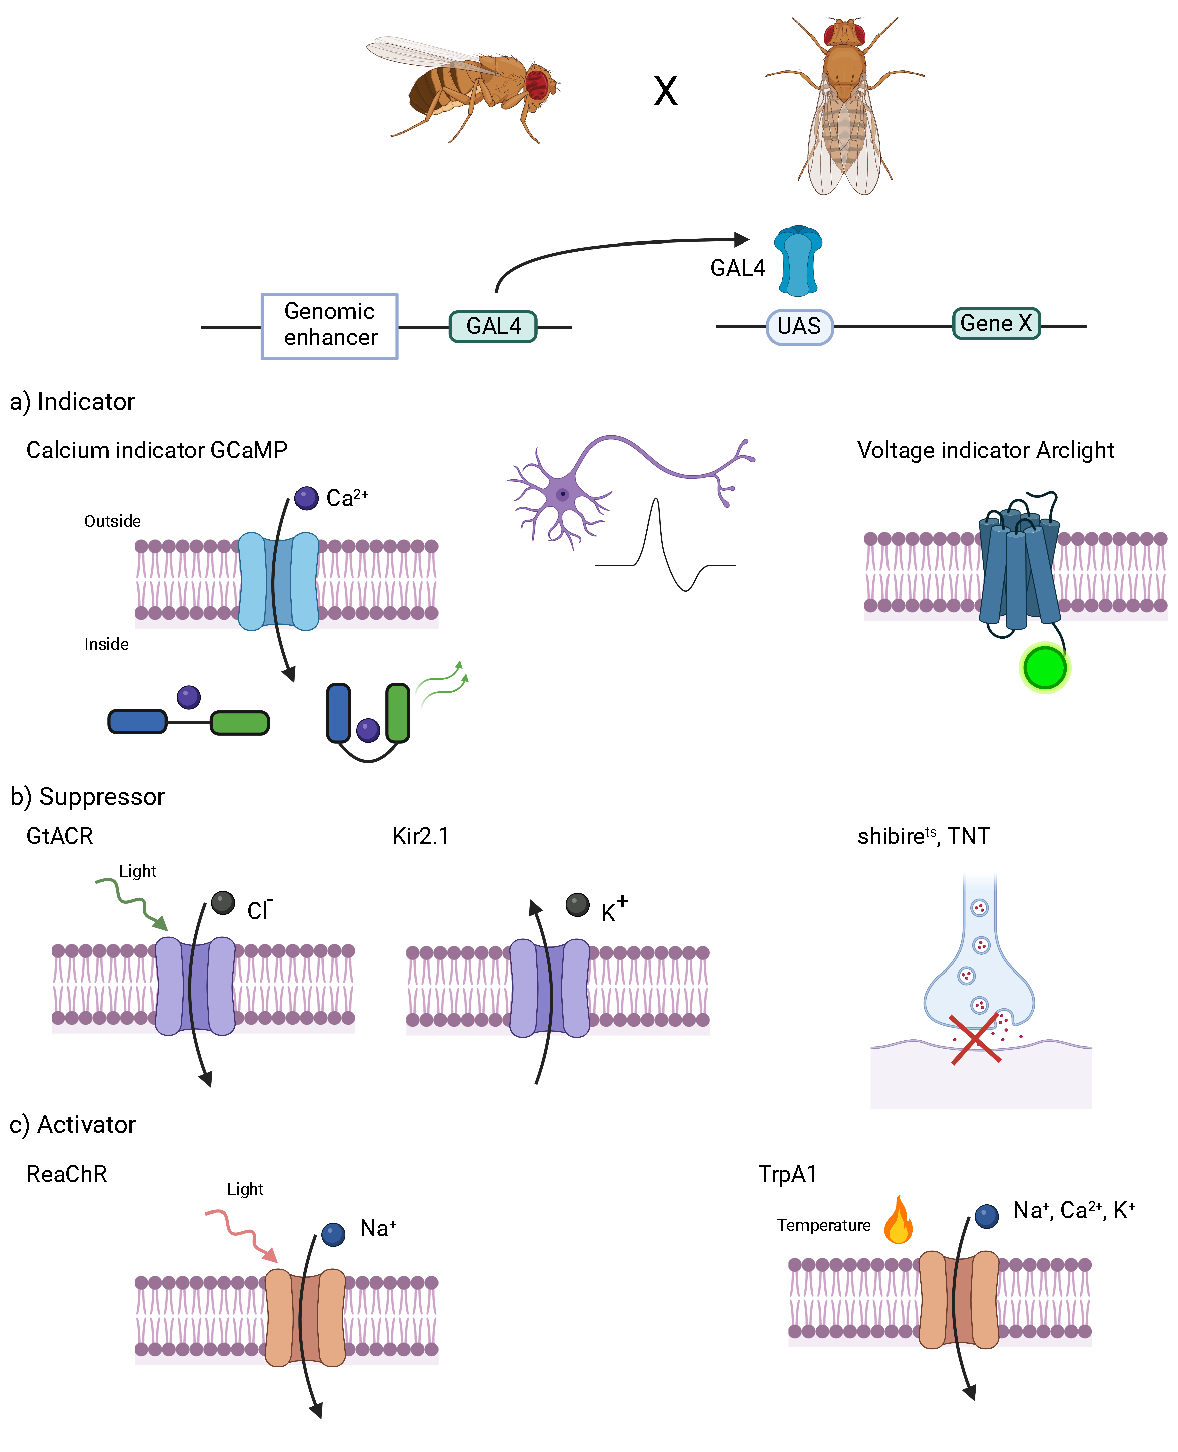
\includegraphics[scale=0.8]{Gal4-UAS}
\caption[Genetic tools for functional manipulations in \textit{Drosophila}] {The Gal4-UAS system is used to express a gene of interest in a specific subset of neurons. (a) The calcium indicator is used to record neural activity using intracellular calcium concentration. The voltage indicator is used to optically record membrane potential changes in the neuron. (b) Neural activity can be suppressed by expressing light-sensitive chloride channels, overexpression of potassium channels resulting in potassium efflux or by blocking synaptic transmission. (c) Neurons can be activated via the expression of light-sensitive or tempearture-sensitive cation channels. (modified from \cite{Borst2009})}
\label{fig:gal4uas}
\end{figure}

\subsection{Measuring neural activity}
\paragraph{Electrophysiology}
Electrophysiological recordings are used to measure neural activity by recording voltage or current changes across the neuronal membrane at a high temporal resolution. Depending on where the electrode is placed in relation to the cell, electrophysiological recordings can be classified into three main types: (1) extracellular recordings; (2) intracellular recordings; and (3) patch-clamp recordings. The large membrane voltage changes during an action potential causes local, temporary differences in potential in the extracellular space near the membrane of an active neuron. In extracellular recordings, an electrode is placed in the vicinity of the neuron to record these extracellular voltage changes. In insects, however, neurons often do not fire action potentials, but rather use graded potentials \parencite{Haag1998}. In the blowfly \textit{Calliphora erythrocephala}, intracellular recordings using a sharp electrode were used to characterize the large lobula plate tangential cells \parencite{Hausen1976, Krapp1998}.

The small size of \textit{Drosophila} neurons makes sharp electrode recordings difficult. The third variant, the whole-cell patch-clamp recordings were found to be better suited \parencite{Hamill1981}. The patch-clamp method involves making tight contact with a tiny patch of the neuronal membrane with a glass micropipette. By briefly applying strong suction to the pipette, the membrane patch within it can be disrupted and the interior of the pipette can be continuous with the cytoplasm. In this configuration, electrical potentials and currents are measured from the entire cell, thus the method is called whole-cell recording. Several brain areas, including the visual \parencite{Groschner2022, Gruntman2018, Joesch2008, Behnia2014} and olfactory systems \parencite{Wilson2004}, have been recorded \textit{in vivo} using patch-clamp techniques in \textit{Drosophila}.
\paragraph{Two-photon microscopy}
Although electrophysiology is widely used to record action potentials and sub-threshold changes in membrane potential, it has significant disadvantages. Electrodes must be inserted into the neurons or the brain tissue. This can cause cell or tissue damage. Additionally, only a limited number of neurons can be recorded simultaneously. With the advent of silicon probe technology, which allows multiple probes to be inserted into the brain (each with hundreds of contact points), a greater number of neurons and brain regions can be sampled using electrophysiology. However, these recordings are more invasive, more expensive, and have the same limitations as single-neuron electrode recordings. Optical probing of neural activity, especially combining calcium or voltage imaging with two-photon microscopy has become popular as an alternative to electrophysiology. 

The invention of two-photon microscopy \parencite{Denk1990} has been one of the major breakthroughs in neuroscience. It allows high-sensitivity and high-resolution fluorescence detection in brain tissue \textit{in vivo}. In two-photon microscopy, two low-energy near-infrared or infrared photons (usually from the same laser) cooperate to produce an electronic transition in a fluorescent molecule from the ground to the excited state. In other words, a fluorescent molecule can achieve a higher energy state either by absorbing a single photon from 455 nm light or by absorbing two photons simultaneously from a light of wavelength 910 nm. Compared to one-photon techniques, two-photon excitation provides several advantages for microscopy in scattering specimens like the brain \parencite{Denk1994, Svoboda2006}. First, compared to the visible wavelengths used in one-photon microscopy, the near-infrared or infrared excitation wavelengths used in two-photon microscopy penetrate the tissue better. This happens due to the reduced scattering and reduced absorption by endogenous chromophores. Second, the bleaching of fluorophores is reduced in two-photon imaging compared to one-photon imaging. Fluorophores lose their brightness when exposed to high-energy light. Light of higher wavelength used in two-photon microscopy carries less energy and hence, causes reduced bleaching. Third, the light above 900nm in the infrared region is beyond the spectral sensitivity of a fly’s eye. Hence, the laser light won’t interfere with the light used to create visual stimuli. Combining two-photon microscopy with a precise genetic expression of genetically encoded calcium indicators (GECIs) \parencite{Chen2013} has been extensively used to measure neural activity in \textit{Drosophila} neuroscience. 

\paragraph{Two-photon calcium imaging}
\textit{In vivo} two-photon calcium imaging is based on the principle that when neurons are sufficiently depolarized, intracellular calcium rise, which can be detected using GECIs that bind to calcium (figure \ref{fig:gal4uas}a). GECIs typically consist of a calcium-binding domain - calmodulin, calmodulin-binding peptide M13, and a reporter element which is based on either a single fluorescent protein or two fluorescent proteins \parencite{Broussard2014}. In the case of a single fluorescent protein for example in GCaMPs, calmodulin (CaM) binds to the M13 peptide in the presence of calcium. This coupling results in conformational changes in the fluorescent protein, resulting in a change in fluorescence intensity \parencite{Nagai2001}.

Two-photon calcium imaging provides several advantages over electrophysiology. First, two-photon calcium imaging is less invasive. Second, it can be combined with genetic tools (for example, Gal4-UAS, LexA-lexAop), to precisely target and record from a specific subset of neurons. Third, two-photon calcium imaging allows recording from several neuronal compartments including soma, dendrites, axons, or single spines and boutons \parencite{Grienberger2022}. In this thesis, I used GCaMP6f  \parencite{Chen2013} in combination with two-photon microscopy for recording neural activity.

\paragraph{Two-photon voltage imaging}
Despite the many advantages that two-photon calcium imaging offer, there are some disadvantages. Calcium imaging does not reveal inhibitory, hyperpolarizing signals. Also, calcium imaging is limited on the temporal scale. It is possible to overcome the limitations inherent in calcium imaging with optical voltage imaging. The genetically encoded voltage indicators (GEVIs) consist of a voltage-sensing domain fused together with a fluorescent protein. The coupling of voltage sensing with optical output is achieved either via Förster resonance energy transfer (FRET) between fluorescent proteins (FPs) or by sensitizing a single fluorescent protein by circular permutation. 

The voltage indicators produce weak optical signals compared to calcium indicators GCaMPx, which is why few system neuroscience studies have been conducted on them. However, the potential of GEVIs is very high, and therefore a lot of effort is being put into improving the existing GEVIs and also developing new ones. Due to the low signal amplitude, experiments with optical voltage indicators such as ASAP2f have been challenging \parencite{Yang2016}. In this thesis, I used a fluorescence protein voltage sensor called Arclight \parencite{Jin2012}. Arclight is based on the fusion of the voltage sensing domain of \textit{Ciona intestinalis} voltage-sensitive phosphatase \parencite{Murata2005} and the fluorescent protein super ecliptic pHluorin with an A227D mutation. Arclight's fluorescence decreases with membrane depolarization and increases with membrane hyperpolarization. Arclight has been shown to robustly report both subthreshold events and action potentials in genetically targeted neurons in the intact \textit{Drosophila} brain \parencite{Cao2013}. I used Arclight in combination with two-photon imaging to record changes in the neuronal membrane potential.

\subsection{Manipulating neural activity}

The above-mentioned tools are suitable for measuring the neural activity and characterizing a neuron. It is necessary, however, to also activate or silence a neuron in order to investigate its functional contribution to the neural circuit. 

\paragraph{Silencing neurons}
There are several genetic tools that allow for silencing neurons in \textit{Drosophila} (figure \ref{fig:gal4uas}b). First, the cell death genes such as \textit{reaper (rpr)} or \textit{head involution defective (hid)} can be expressed to induce apoptosis and kill the neurons \parencite{Chen1996, Grether1995}. Second, the synaptic output of neurons can be permanently blocked. The \textit{tetanus toxin light chain (TNT)} cleaves the synaptic vesicle protein synaptobrevin and inhibits neurotransmitter exocytosis at chemical synapses \parencite{Sweeney1995}. Third, the expression of \textit{Kir2.1} -- an inwardly rectified potassium channel, can cause neurons to constantly hyperpolarize, resulting in suppressed excitability \parencite{Johns1999}. While using the Gal4-UAS system to express these effector proteins provides effective control over the functionality of the targeted neurons, their expression cannot be reversed and the precise timing of silencing the neurons cannot be determined. To overcome these limitations, the conditional effector proteins like \textit{$shibire^{ts}$} \& \textit{GtACR}, which is activated by higher temperature and light respectively can be used. 

The \textit{Drosophila} gene \textit{shibire} encodes the protein \textit{dynamin}, which is involved in the process of endocytosis and is essential for vesicle recycling. The dominant-negative temperature-sensitive allele $shibire^{ts}$ is defective in synaptic vesicle recycling at the restrictive temperature (${>}29\degree C$). The reuptake of vesicles from the synaptic cleft, mediated by the GTPase dynamin, is still functional at a permissive temperature (${\sim}25\degree C$). Thus, a rapid and reversible inhibition of synaptic transmission can be achieved by controlling the temperature of the specimen \parencite{Kitamoto2001}. As an alternative to temperature, light can be used to control the timing of silencing the neuron. Light-gated anion channel, \textit{Guillardia theta} anion channel rhodopsins (GtACR) can be expressed in the neurons of interest. The application of light causes these channels to open, allowing an influx of chloride ions, thus causing the neurons to hyperpolarize. This is an extremely sensitive, precisely timed, and reversible method for manipulating neural activity \parencite{Govorunova2015, Mauss2017, Mohammad2017}.

\paragraph{Activating neurons}
A second or complementary approach to probing the functional role of a neuron in a neural circuit is by activating the neuron (figure \ref{fig:gal4uas}c). Temperature-sensitive channels can be used for activating the neurons. Flies naturally express the transient receptor potential cation channel TrpA1 which is implicated in temperature detection \parencite{Hamada2008, Pulver2009}. The expression of these channels in the neurons allows for temperature-mediated excitation. The light-gated optogenetic tools, however, allow for greater temporal control compared to the above-mentioned temperature-sensitive method. The light-gated cation channel \textit{Channelrhodopsin (ChR)} was extracted from the green algae \textit{Chlamydomonas reinhardtii} and expressed in \textit{C. elegans} and mammalian hippocampal neurons \parencite{Nagel2005, Boyden2005}. By expressing these light-gated cation channels in the neurons of interest, a precise, reversible, and reliable excitation of the neurons can be achieved.

\section{Neural communication}
Camillo Golgi's silver-stain method made it possible for the first time, to visualize single neurons in tissue samples under the light microscope (1873). Santiago Ramón y Cajal in 1888 described the nervous system as a network of individual cells. About a decade later, in 1897, the term 'synapse', derived from the Greek word 'synapsis' (meaning 'conjunction'), was used to describe the connections between two neurons. Neurons form networks where they communicate via synapses. Two types of synapses exist 1) electrical synapses and 2) chemical synapses.

\subsection{Electrical synapses}
In electrical synapses, two cells are directly connected by a cluster of intercellular channels called gap junctions \parencite{Bennett2004}. The gap junctions provide a conductive pathway for electrical current to spread between cells. Consequently, electrical currents underlying action potentials or graded potentials directly propagate to postsynaptic neurons, without additional delay. Since electrical signals propagate bidirectionally, signalling events generated in the postsynaptic cells can also spread to presynaptic cells. In \textit{Drosophila}, electrical synapses are widely distributed throughout the nervous system and are essential to neuronal function \parencite{Ammer2022, Stebbings2002, Liu2016}.

\subsection{Chemical synapses}
Neurons communicate mostly via chemical synapses (figure  \ref{fig:chemicalsynapse}). When the presynaptic membrane is sufficiently depolarized, voltage-gated calcium channels open and allow $Ca^{2+}$ to enter the cell \parencite{Luo2020}. Calcium entry leads to the fusion of synaptic vesicles with the membrane and the release of neurotransmitter molecules into the synaptic cleft \parencite{Chapman2002}.  As neurotransmitters diffuse across the synaptic cleft, they bind to receptors in the postsynaptic membrane, causing the postsynaptic neuron to depolarize or hyperpolarize, thereby passing the information from pre- to postsynaptic neurons \parencite{Maio2008}. 

\begin{figure}
\centering
\hspace*{-1cm} 
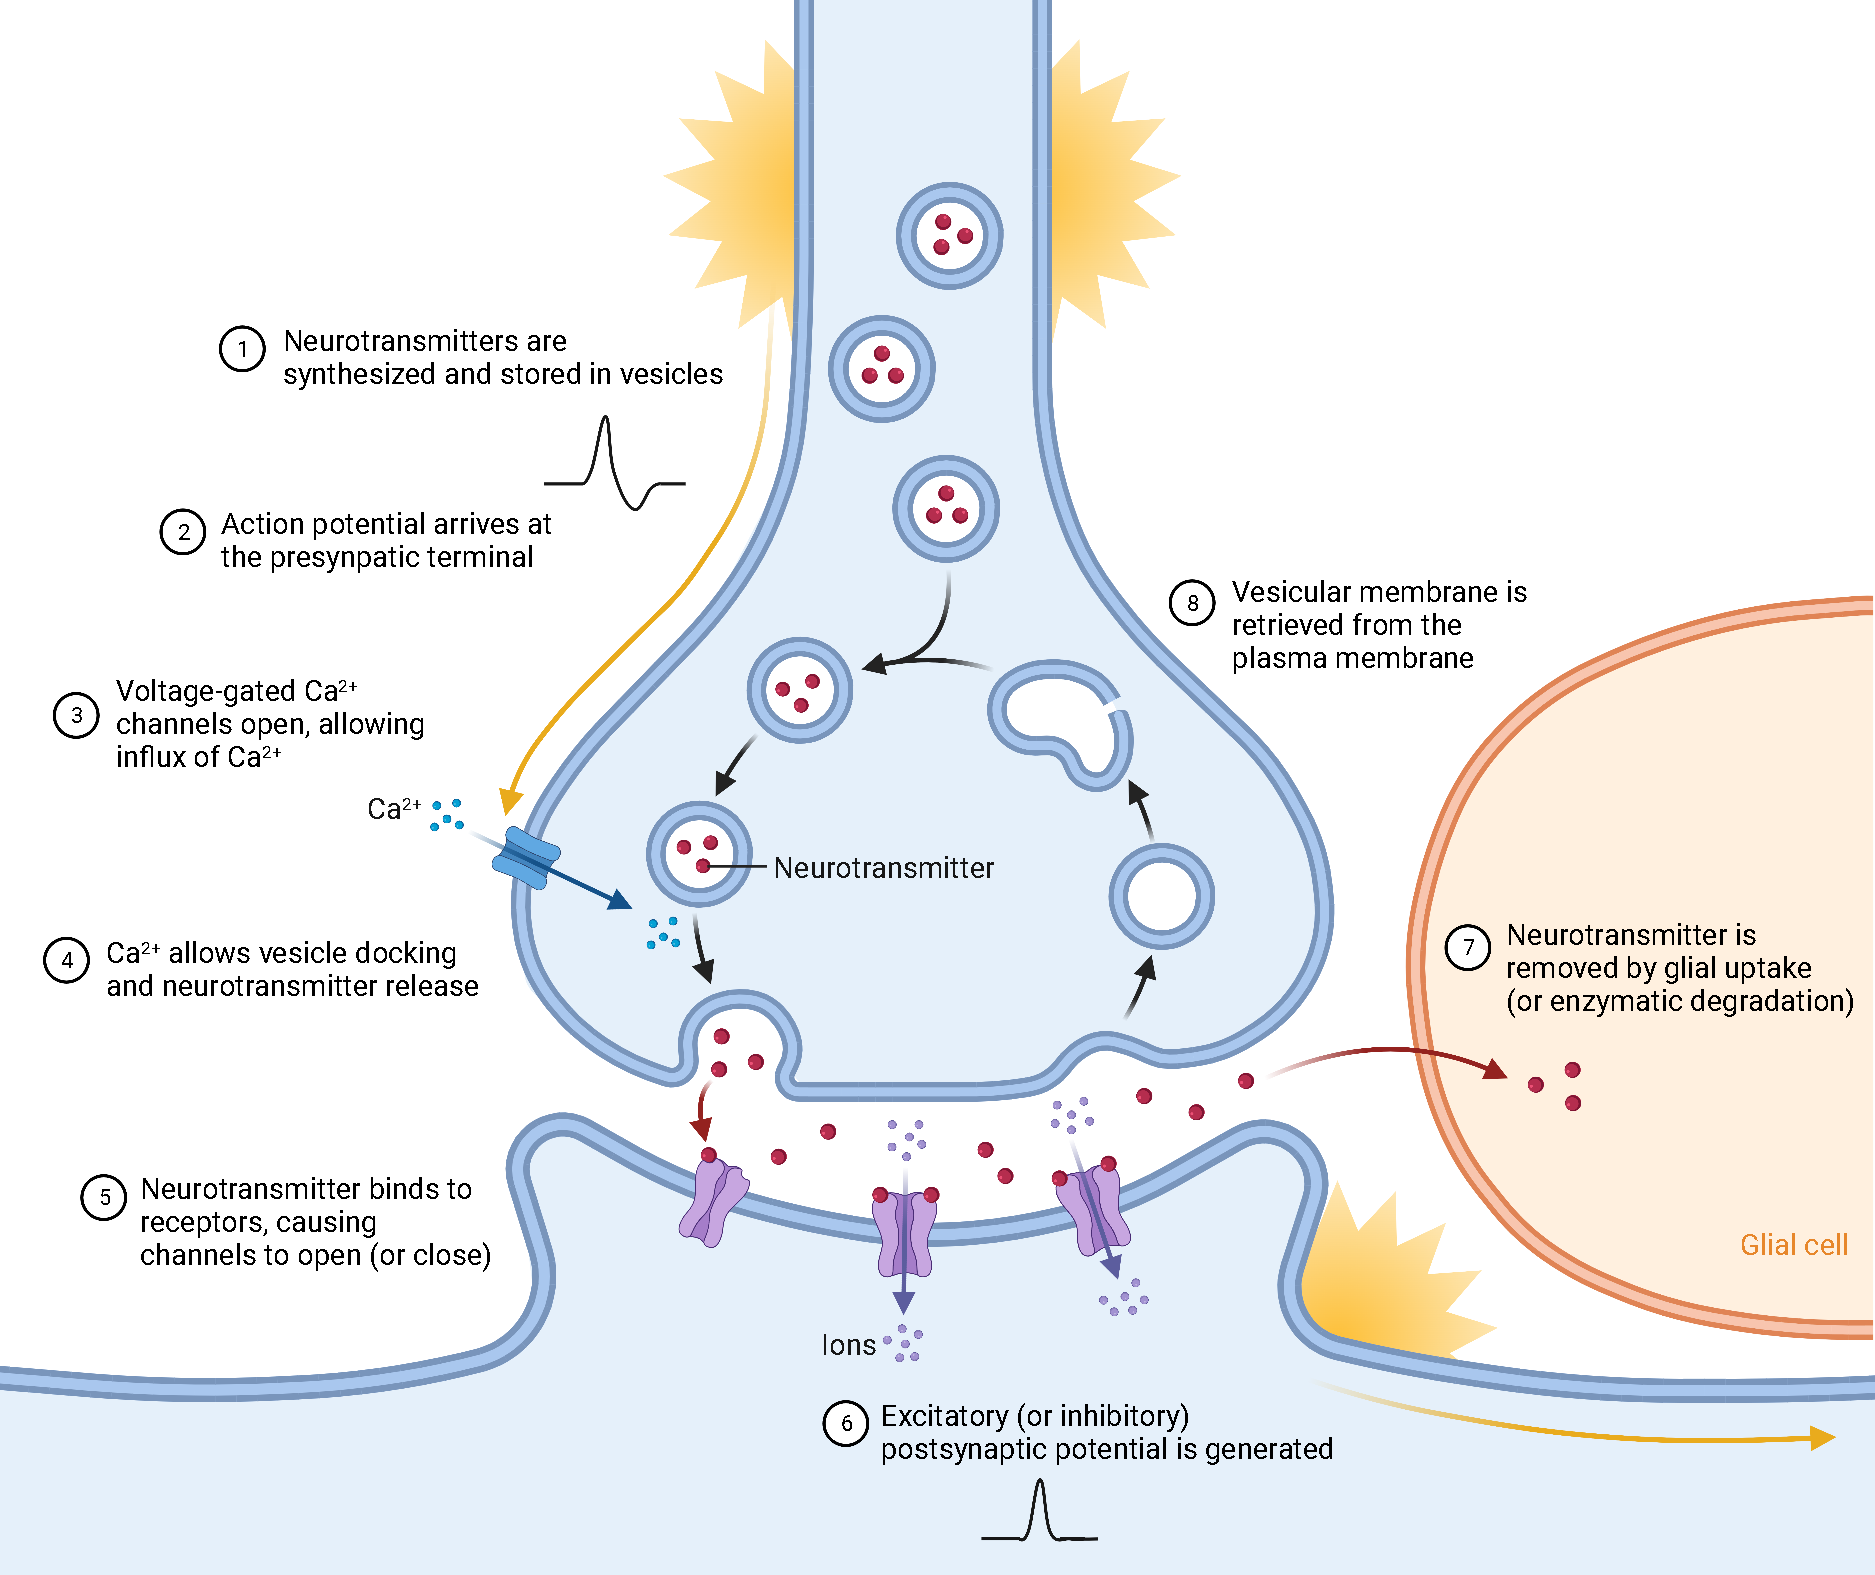
\includegraphics[scale=0.29]{Chemical_Synapse}
\caption[Chemical synapse: steps of synaptic transmission] {Chemical synapse: steps of synaptic transmission. (1) Synthesis and storage of neurotransmitters in the vesicles. (2) Depolarization in the presynaptic terminal causes (3) voltage-gated calcium channels to open and allow an influx of calcium ions. (4) High concentration of calcium ions triggers the fusion of neurotransmitters-filled vesicles with the presynaptic membrane and the release of neurotransmitters into the synaptic cleft. (5) Neurotransmitters released in the synaptic cleft bind to receptors in the postsynaptic membrane leading to (6) excitatory or inhibitory postsynaptic potential. (figure created with \href{https://app.biorender.com/biorender-templates}{Biorender.com})}
\label{fig:chemicalsynapse}
\end{figure}

\subsection{Voltage-gated ion channels}
Voltage-gated ion channels are transmembrane proteins that allow certain inorganic ions to cross cell membranes (figure  \ref{fig:vgatedionc}). Generally, these channels consist of two distinct but functionally coupled transmembrane domains: the voltage sensing domain and the pore domain. The voltage sensing domain changes the conformation of the pore domain in response to changes in transmembrane potential, allowing selected ions to flow down their electrochemical gradient. 

\paragraph{Voltage-gated calcium channels}
As mentioned above, voltage-gated calcium channels mediate depolarization-induced calcium influx that drives the release of neurotransmitters. The $\alpha1$-subunit of the voltage-gated calcium channels forms the ion-conducting pore, which makes it distinct from other calcium channels. Three families of genes encode $\alpha1$ subunits. \textit{Drosophila} genome has one $\alpha1$ subunit gene in each family: $\alpha1D$ ($Ca_{v}1$), cac ($Ca_{v}2$), and $\alpha1T$ ($Ca_{v}3$) \parencite{Littleton2000, King2007}. In \textit{Drosophila} antennal lobe projection neurons, cac ($Ca_{v}2$) type and $\alpha1T$ ($Ca_{v}3$) type voltage-gated calcium channels are involved in sustained and transient calcium currents, respectively \parencite{Gu2009, Iniguez2013}.

\paragraph{Voltage-gated sodium channels}
In neurons, voltage-gated sodium channels play a crucial role in the initiation and propagation of action potentials \parencite{Hodgkin1952}. Sodium channels are activated and deactivated within milliseconds when the membrane is depolarized by a few millivolts. There are at least ten genes in mammals that encode these large membrane proteins. In contrast, \textit{paralytic (para)} is the only voltage-gated sodium channel gene described in \textit{Drosophila} \parencite{Piggott2019}. %Loss of \textit{paralytic (para)} reduces neuroblast progeny cell number in \textit{Drosophila} \parencite{Piggott2019}.

\paragraph{Voltage-gated potassium channels}
Voltage-gated potassium channels are transmembrane channels specific to potassium ions. They play a crucial role in repolarizing the depolarized cell to its resting membrane potential, after each action potential. Voltage-gated potassium channels are the most diverse family of voltage-gated ion channels in the human genome, with 40 members for $\alpha$ subunit grouped into 12 families \parencite{Gutman2005}. The first voltage-gated potassium channel discovered in \textit{Drosophila} was \textit{Shaker} \parencite{Papazian1987}. Afterwards, three additional \textit{Shaker} like voltage-gated potassium genes were identified: \textit{Shab}, \textit{Shaw} and \textit{Shal} \parencite{Covarrubias1991}. 

\begin{figure}
\centering
\hspace*{-1cm} 
\includegraphics[scale=0.85]{voltagegatedionchannels}
\caption[Voltage-gated ion channels] {Voltage-gated ion channels: The sodium channels allow $Na^{+}$ ions to enter the cell. The calcium channels allow $Ca^{2+}$ ions to enter the cell. The potassium channels allow efflux of the $K^{+}$ ions.}
\label{fig:vgatedionc}
\end{figure}


\section{The fly visual system}

As mentioned earlier, the \textit{Drosophila melanogaster} nervous system consists of ${\sim}200,000$ neurons \parencite{Raji2021}. Almost half of these neurons (${\sim}100,000$ neurons) are dedicated to processing visual signals in the optic lobe of the fly brain. Unlike vertebrates, many invertebrate species have compound eyes, which are composed of multiple optical units called facets or ommatidia. Each compound eye contains around 750 ommatidia \parencite{Ready1976}. The ommatidia are arranged in a regular lattice with a 5-degree inter-ommatidia angle \parencite{Land1997}. There are eight different photoreceptors in an ommatidium (R1-R8). A circular arrangement is formed by R1-R6 enclosing the central photoreceptors R7 and R8, which are stacked on top of one another. Due to this arrangement, the photoreceptors in an ommatidium sense incident light from slightly offset positions in space. With this configuration, six photoreceptors in six different adjacent ommatidia that possess identical optical axes project their axons to a single cartridge in the brain forming a so-called neuro-ommatidium \parencite{Strausfeld1971}. As a result of this neural superposition principle, the sensitivity increases without compromising the spatial resolution \parencite{Kirschfeld1967}.

\paragraph{Phototransduction}
The process of converting light enrgy into electrochemical signals is called phototransduction. This process occurs in rhabdomeres in the flies photoreceptors. In rhabdomeres, there are ${\sim}30,000$ microvilli, each containing about 1000 photoactive molecules, called rhodopsin. The chromophore 3-hydroxy-11-cis-retinal is covalently bound to rhodopsin. Upon absorption of a photon by rhodopsin, the chromophore 3-hydroxy-11-cis-retinal is isomerized to all-trans-retinal, and the activated metarhodopsin state is formed. This activates a G-protein coupled cascade that results in the activation of phospholipase C (PLC). The PLC hydrolyzes phosphatidyl-inositol 4,5 bisphosphate (PIP2) to diacylglycerol (DAG), inositol 1,4,5 trisphosphate (InsP3), and a proton.  Downstream to PLC, two light-sensitive channels (TRP and TRPL) are activated, allowing sodium and calcium to enter the cell and depolarize it. The photoreceptors upon activation release the inhibitory neurotransmitter histamine, thus inhibiting postsynaptic neurons \parencite{Hardie2001, Hardie1989, Hardie2015}.

\begin{figure}
\centering
\hspace*{-1cm} 
\includegraphics[scale=0.75]{fly_optic_lobe}
\caption[The fly optic lobe] {The fly optic lobe: (a) The horizontal cross-section of a reduced silver stain shows the columnar organization of the retina (R), lamina (L), external chiasm (EC), medulla (M), internal chiasm (IC), lobula (Lo), and lobula plate (Lp). Scale bar = $50 \, \mu m$. Reproduced, with permission, from \cite{Takemura2008} (b) Schematic illustration of direction selectivity: moving a bar in front of a fly's eye leads to depolarization of photoreceptors every time, regardless of whether the bar moves to the right or left. It is a non-directional signal. A few synapses downstream, on the lobula plate tangential cells, signals are direction-selective: these cells depolarize during movement along one direction, i.e., their 'preferred' direction, and hyperpolarize during motion along the opposite direction, i.e., their 'null' direction. (c) An overview of all types of columnar cells in the \textit{Drosophila} optic lobe. (\cite{Fischbach1989}) (d) Columnar cell types involved in the motion vision circuit. (Used with permission from \cite{Borst2020, Borst2020b})}
\label{fig:opticlobe}
\end{figure}

\subsection{The optic lobe}

Following the photoreceptor layer in the retina, the fly’s optic lobe consists of 4 layers of neuropils called the lamina, the medulla, the lobula, and the lobula plate. These neuropil layers are arranged in a columnar, retinotopic fashion with each column processing information from a small point in the visual space (figure \ref{fig:opticlobe}a) \parencite{Fischbach1989}.

\paragraph{Lamina}
The lamina is organized in an array of ${\sim}750$ retinotopic columns (also called 'cartridges'). Each column corresponds to ${\sim}5\degree$ discrete sample of the visual world. The light-sensitive photoreceptors, R1-6 project their axons into each lamina column. Two other photoreceptors, R7 \& R8 pass through the lamina and synapse in specific layers of the medulla. Along with photoreceptor axons, the lamina includes 5 lamina output neurons (L1-L5), six putative feedback neurons (T1, Lat, Law1, Law2, C2, C3), and one lamina intrinsic neuron (Lai). L1, L2, and L3 cells receive the majority of their input from photoreceptors R1-R6. L4 cells form reciprocal connections with L2 and receive only a small number of input from photoreceptor R6. L5 receives input from L2, L4, and lamina interneurons \parencite{Rivera2011}. The lamina columnar monopolar neurons, L1-L5 send their axonal projections into specific layers of the medulla. \parencite{Fischbach1989, Tuthill2013}. Lamina output neurons L1 and L2 are the primary input cells for motion vision \parencite{Zhu2013}.

\paragraph{Medulla}
Lamina cells send input projections to the medulla, the second neuropil in the optic lobe. There are ten synaptic layers (M1 to M10) in the medulla consisting of over 60 types of cells. The medulla is composed of hexagonal columns, similar to the lamina. In this way, the mapping between the lamina and medulla remains retinotopic. The fibers connecting the lamina to the medulla form a chiasm, in which posterior medulla cartridges receive input from anterior lamina cartridges. Two main classes of columnar interneurons are found in the medulla: around 10 types of medulla intrinsic neurons (Mi) and around 30 types of transmedullary neurons (Tm). Mi neurons connect different layers of the medulla to each other. Dendrites of Mi cells are located in the distal medulla layers, while axons are located in the proximal medulla layers. Tm neurons connect specific layers of the medulla to various layers in the lobula. Tm cells receive input in the distal medulla layers 1-5 from lamina monopolar cells and photoreceptors R7 and R8 and send their axonal projections to the lobula \parencite{Fischbach1989, Takemura2011}. In addition to these two types of neurons, the trans-medulla Y ('TmY') neurons connect specific layers of the medulla to various layers in the lobula and lobula plate.

\paragraph{Lobula complex}
In the final stage of the visual processing in the optic lobe, the lobula complex consists of two neuropils: the lobula and the lobula plate. There are six layers in the lobula \parencite{Fischbach1989}. Lobula columnar (LC) neurons receive major inputs from the medulla and are the most prominent type of cell in the lobula. Multiple types of LC neurons span the entire visual field in a retinotopic manner \parencite{Otsuna2006}. In total, these neurons are divided into more than twenty distinct subtypes, each conveying information about a different visual feature \parencite{Wu2016}. Lobula plates have four structurally distinct layers perpendicular to their columnar organization. A number of wide-field tangential cells are present in each layer \parencite{Strausfeld1991}. Dendritic trees of the tangential cells span large areas of the lobula plate, sometimes covering the entire layer. Thus, their receptive fields cover a large portion of the visual field. Two types of bushy T-cells T4 and T5 exist. Four subtypes of both T4 and T5 are found connecting the medulla and lobula respectively to the four layers of the lobula plate \parencite{Fischbach1989}.

\subsection{Neural circuits underlying direction selectivity}
Direction selectivity is the most important response characteristic of the lobula plate tangential cells. In response to a visual stimulus moving in their preferred direction, the cells depolarize. When the visual stimulus moves in the opposite direction (the null direction), the cells hyperpolarize. Two major types of lobula plate tangential cells have been described. The horizontal system (HS) cells respond preferentially to horizontal motion \parencite{Schnell2010}, while vertical system (VS) cells respond preferentially to vertical motion \parencite{Joesch2008}. Photoreceptor signals, in contrast, are not direction-selective, i.e. they display a similar response regardless of which direction the stimulus moves. Thus, a non-directional response at the photoreceptor level is transformed into a directional signal at the lobula plate tangential cell level (figure \ref{fig:opticlobe}b). The lobula plate tangential cells, however, integrate signals over large parts of visual fields, i.e. they are not local motion detectors. Hence, the question arises: which cells are the local motion detectors? 

%If one were to record from a single photoreceptor in the retina, it would show a similar response to moving images irrespective of the direction of motion: meaning it is not direction-selective. However, if one records around 4 synapses downstream, Lobula Plate Tangential Cells (LPTCs) depolarise in response to the image moving in its preferred direction and hyperpolarize if the image moves in the opposite direction or the null direction (figure \ref{fig:opticlobe}b). HS (Horizontal System) cells for example are responsive to horizontal motion \parencite{Schnell2010}, while VS (Vertical System) cells are responsive to vertical motion \parencite{Joesch2008}. LPTCs however, integrate over large parts of visual fields, i.e. they are not local motion detectors. Hence, the question arises: which cells are the local motion detectors? 

%The answer to the above question is: T4 and T5 are the first local motion detectors found in the \textit{Drosophila} ON and OFF motion vision pathway, respectively. Four sub-population of T4a-d and T5a-d cells tuned to the four cardinal directions and projecting to the four layers in the lobula plate can be found within each column \parencite{Maisak2013}. This leads to the next question: what makes T4 and T5 direction selective? To answer this question, we need to investigate the cells which are present between the non-direction-selective photoreceptors in the retina and direction-selective T4, and T5 cells in Medulla and Lobula respectively (figure \ref{fig:opticlobe}c, d). The columnar cell types of the lamina, medulla, lobula, and lobula plate have been identified and described \parencite{Fischbach1989, RamonyCajal1915}.  

%While the cell types in the optic lobe were known, the small size of these neurons made electrophysiological recordings difficult. After the advent of modern two-photon imaging in combination with using the Gal4-UAS system to express GCaMP, it was possible to record neuronal activity from these cells. 
Electrophysiological and two-photon calcium imaging experiments in the optic lobe over the years have revealed the following interesting results: (a) Visual processing in \textit{Drosophila} occurs in two parallel processing pathways for luminance increment (ON) and luminance decrement (OFF) \parencite{Joesch2010, Joesch2013, Strother2014, Eichner2011, Behnia2014, Shinomiya2014} (b) T4 and T5 are the first local motion detectors found in the \textit{Drosophila} ON and OFF motion vision pathway respectively. Four sub-population of T4a-d and T5a-d cells tuned to the four cardinal directions and projecting to the four layers in the lobula plate is found within each column \parencite{Maisak2013}. 


\paragraph{Parallel ON and OFF processing pathways}
In striking similarity to the mammalian retina \parencite{Masland2012}, visual processing in \textit{Drosophila} occurs in two parallel ON and OFF processing pathways \parencite{Borst2015}. The ON pathway transmits information about luminance increments, while the OFF pathway transmits information about luminance decrements. The split into the ON and OFF pathways occurs in the lamina. The L1 neurons provide inputs onto the ON pathway, while the L2 neurons provide inputs onto the OFF pathway. When the output of L1 neurons was genetically blocked, the downstream motion-sensitive lobula plate tangential cells no longer responded to ON motion. Blocking the output of L2 neurons abolished the responses of the tangential cells to OFF motion \parencite{Joesch2010}. In behavioral experiments, walking flies were unable to follow either ON or OFF motion when either L1 or L2 was blocked respectively \parencite{Clark2011, Maisak2013}. The flies became completely motion-blind when both L1 and L2 were permanently hyperpolarized (via \textit{Kir2.1}) \parencite{Tuthill2013, Bahl2013}. These experiments together showed that the L1 neurons specifically transmits information to the downstream ON motion detector, and the L2 neuron specifically transmits information to the downstream OFF motion detector. 

\paragraph{T4 and T5 cells}
Based on previous studies \parencite{Fischbach1989, Buchner1984}, T4 and T5 were long thought to be the prime candidates for local motion detectors in the ON and OFF pathways respectively. However, due to its small size, it was difficult to do electrophysiological recordings from T4 and T5 cells \parencite{Douglass1996}. This problem was solved using a combination of two-photon imaging and a Gal4-UAS system to express GCaMP in T4, and T5 cells to record its neural activity in response to the ON and OFF stimuli. Stimulating the flies with visual motion in four cardinal directions (front-back, back-front, upwards, and downwards), direction-selective activity from T4/T5 cells were recorded \parencite{Maisak2013}. Four sub-populations of T4a-d and T5a-d cells tuned to the four cardinal directions and projecting to the four layers in the lobula plate were found within each column. Further, the T4 cells were found to respond specifically to ON stimulus and the T5 cells were found to respond specifically to OFF stimulus. Blocking T4 and T5 cells led to a complete loss of motion response in the lobula plate tangential cells \parencite{Schnell2012}, and of the optomotor response of tethered walking flies \parencite{Bahl2013}. Specific blocking of T4 cells led to a reduction in tangential cells and optomotor responses to ON stimulus selectively, while specific blocking of T5 cells led to a reduction in tangential cells and optomotor responses to OFF stimulus selectively. These results together show T4 and T5 cells to be the elementary motion detector for the ON and OFF pathways respectively \parencite{Maisak2013}.    

\begin{figure}
\centering
\hspace*{-1.4cm} 
\includegraphics[scale=0.15]{t4t5inputsynapses}
\caption[Synaptic sites distributed over T4 and T5 dendritic arbors]{Synaptic sites distributed over T4 and T5 dendritic arbors: An arbor of a T4c (top panels) or T5c (bottom panels) cell is shown with synapse positions plotted on the dendritic arbors. Unless shown as 'Presynapse', puncta are postsynaptic sites (input to T4/T5 cells). T4c and T5c detect upward motion, and other subtypes of T4 and T5 cells show similar distribution patterns (not shown). An arbor's first branch point is indicated by pink stars. (Used with permission from \cite{Shinomiya2019})}
\label{fig:t4t5inputsynapses}
\end{figure}  

%\section{Neural circuit underlying direction selectivity}
Having identified T4 and T5 cells as elementary local motion detectors, the next question is which cells provide synaptic inputs to these cells. Electron Microscopy (EM) studies \parencite{Shinomiya2019, Takemura2017} provided the answer to this question. FIB-SEM (Focused Ion Beam Scanning Electron Microscopy) was used to record a volume of the optic lobe comprising seven columns of the medulla, lobula, and lobula plate \cite{Shinomiya2019}. All the different neuron types providing inputs to the T4 and T5 cells were identified. T4 cells receive input from Mi1, Tm3, Mi4, Mi9, C3, CT1, and TmY15. T5 cells receive input from Tm1, Tm2, Tm4, Tm9, CT1, TmY15, LT33, and Tm23. The T4 and T5 cells' dendrites span several columns along the preferred direction of the motion. The location where the different cell types synapse onto the dendrites of T4 and T5 was also found. For example, a T4c cell with the preferred direction of motion as upwards receives input from Mi1, Tm3, and TmY15 in the central part of its dendrite, from Mi9 and T4c on the ventral part, and from Mi4, C3, and CT1 on the dorsal part of its dendrite [figure \ref{fig:t4t5inputsynapses} top]. T4d cells with preferred direction as downwards receive input from Mi1, Tm3, and TmY15 in the central part, from Mi9 and T4d on the dorsal part, and from Mi4, C3, CT1 on the ventral part of its dendrite. In summary, all T4 subtypes receive inputs from Mi1, Tm3, and TmY15 in the central part, from Mi9 on the preferred side (i.e. the side from which a preferred direction stimulus approaches), and from Mi4, C3, and CT1 on the null side (i.e. the side from which a null direction stimulus approaches) of their dendrite. Similarly, all T5 subtypes receive inputs from Tm1, Tm2, and Tm4 on the central part, Tm9 on the preferred side, and CT1 on the null side of their dendrite [figure \ref{fig:t4t5inputsynapses}]. %a figure showing summary of different inputs.    

Most of these input elements have been characterised physiologically \parencite{Arenz2017, Serbe2016, Strother2017, Meier2019, Behnia2014, Groschner2022}. None of these cells were found to be direction-selective. Hence, the T4 and T5 cells are the elementary motion detector found in the ON and OFF pathway respectively, and thus represents an important processing stage where the direction is computed.    

\subsection{Neural algorithms underlying direction selectivity}
Different models have been proposed to explain the neural computations involved in motion detection. In order to detect motion in a directionally selective manner, local motion detection mechanisms must meet certain minimum requirements \parencite{Borst1989}:
\begin{enumerate}
\item Spatial offset: Motion is a vector that needs two points to be represented, so at least two spatially separated inputs are required.
\item Temporal asymmetry: There must be at least one input that is delayed. If not, the input signals arrive in the subsequent stage simultaneously independent of the stimulus direction.
\item Non-linear interaction: It is necessary to integrate the input signals nonlinearly at a subsequent stage of the process. In the absence of this, the detector's output would be equal for both directions on average.
\end{enumerate} 

\begin{figure}
\centering
\hspace*{-1cm} 
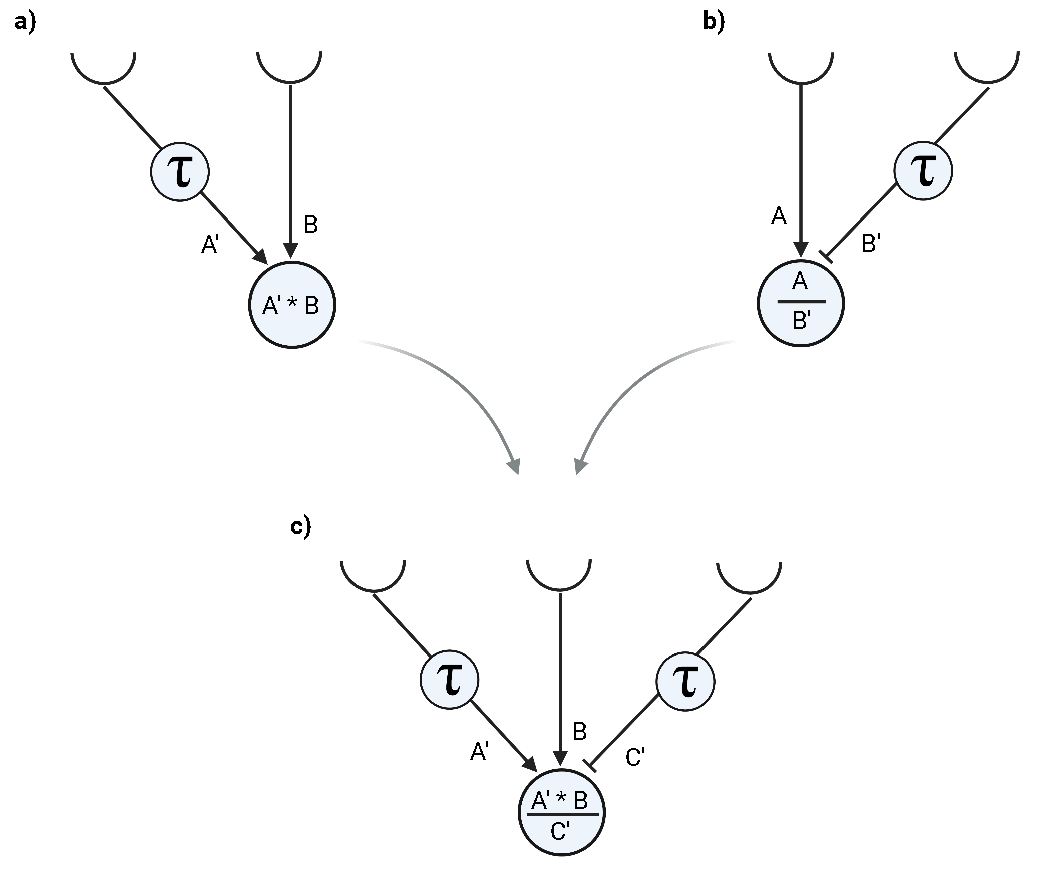
\includegraphics[scale=0.4]{HRBL_model}
\caption[Models for motion detection] {Models for motion detection: (a) The Hassenstein-Reichardt (HR) correlator (half-detector shown here) consists of two arms. Motion in the preferred direction (PD) causes two signals from neighboring photoreceptors to coincide due to a delay ($\tau$) on the first arm. There is an enhancement in PD resulting from a multiplicative non-linearity. (b) The Barlow-Levick (BL) detector has the delay on the opposite arm, and the non-linearity is inhibitory, resulting in a null-direction (ND) suppression. (c) Hybrid detector consisting of one HR unit and one BL unit: Three points in space are sampled. There is a time delay ($\tau$) on the outer two arms. The input signals from detector arms A and B are multiplied and divided by the signal from detector arm C in the following stage. Consequently, the signal in the preferred direction is enhanced and the signal in the null direction is suppressed.}
\label{fig:hrblmodel}
\end{figure}

Classically two opposing models have been proposed for the implementation of direction selectivity. Both these models use two input lines, where one of the input lines has been asymmetrically delayed compared to the other, followed by a non-linear interaction. The Hassenstein-Reichardt (HR) model proposes a Preferred Direction (PD) enhancement: the signal on the preferred side is delayed and is subsequently amplified using multiplication of the signal from the other input line (figure \ref{fig:hrblmodel}a) \parencite{Hassenstein1956}. The Barlow-Levick (BL) detector, however, proposes a Null Direction (ND) suppression: the signal on the null side is delayed and divides the signal from the other input resulting in suppression (figure \ref{fig:hrblmodel}b) \parencite{Barlow1965}. \cite{Haag2016} used apparent motion stimuli to show that both the mechanisms i.e. PD enhancement on the preferred side and ND suppression on the null side are used by T4c and T5c cells to produce a direction-selective response (figure \ref{fig:hrblmodel}c). Is that special to upward-tuned T4c cells or is it general for all subtypes of T4 and T5 cells. In the first manuscript \ref{sct:manuscript_haag_mishra} \parencite{Haag2017}, we showed that all four subtypes of T4 and T5 indeed use both PD enhancement and ND suppression to produce direction-selective responses. Therefore, we proposed a new model combining both PD enhancement on the preferred side and ND suppression on the null side. What are the neural correlates implementing these mechanisms? 

The model requires a fast input at the center, slow input providing excitation on the preferred side, and slow input providing suppression on the null side. Interestingly, from the anatomical and functional characterization of the input data discussed earlier, the input neurons for T4 cells providing these three kinds of inputs can be predicted. Mi1 is a fast neuron providing input at the central part of the dendrite, thus a candidate for central fast input. Mi9 is a slow neuron providing input on the preferred side of the dendrite, hence a candidate for input on the preferred side. Mi4, C3, and CT1 are slow neurons providing input on the null side of the dendrite \parencite{Arenz2017}. 

In addition to the synaptic mechanisms on the dendrites of T4 cells described above, further processing in the T4 neurons– voltage to calcium transformation or calcium to neurotransmitter release, can enhance or decrease the direction selectivity of the output signals of T4 cells. Also, using two-photon voltage and calcium imaging in T5 neurons, \cite{Wienecke2018} showed that linear spatial summation is sufficient for the emergence of direction selectivity in T5 cells and that the preferred direction enhancement and null direction suppression in the calcium signal can arise from the non-linear voltage-to-calcium transformation. To better understand the voltage-to-calcium transformation, we compared voltage and calcium signals in T4 cells in the second manuscript \ref{sct:manuscript_mishra_haag}, using two-photon voltage imaging and calcium imaging recordings. We found that the voltage to calcium transformation in T4c neurons enhances their direction selectivity across different stimuli conditions.  






